\documentclass[11pt]{article}

\usepackage[margin=1in]{geometry}
\usepackage[T1]{fontenc}
\usepackage[utf8]{inputenc}
\usepackage{lmodern}
\usepackage{microtype}
\usepackage{amsmath,amssymb,amsfonts,amsthm,mathtools}
\usepackage{enumitem}
\usepackage{xcolor}
\usepackage{tikz}
\usetikzlibrary{arrows.meta,positioning,calc,fit,backgrounds,decorations.pathreplacing,shapes.geometric}
\usepackage{hyperref}
\usepackage[nameinlink,capitalise,noabbrev]{cleveref}

\hypersetup{
  colorlinks=true,
  linkcolor=blue!50!black,
  citecolor=blue!50!black,
  urlcolor=blue!50!black
}

\definecolor{leftblue}{RGB}{38,115,185}
\definecolor{triorange}{RGB}{221,120,37}
\definecolor{rightred}{RGB}{190,55,65}
\definecolor{rootpurple}{RGB}{105,70,160}
\definecolor{softgray}{RGB}{245,246,248}
\definecolor{darkgreen}{RGB}{40,135,95}
\definecolor{softgreen}{RGB}{220,245,235}
\definecolor{softblue}{RGB}{225,238,250}
\definecolor{softorange}{RGB}{252,236,218}
\definecolor{softpurple}{RGB}{238,232,248}

\newtheorem{theorem}{Theorem}[section]
\newtheorem{lemma}[theorem]{Lemma}
\newtheorem{proposition}[theorem]{Proposition}
\newtheorem{corollary}[theorem]{Corollary}
\newtheorem{definition}[theorem]{Definition}
\newtheorem{remark}[theorem]{Remark}
\newtheorem{assumption}[theorem]{Assumption}

\let\hom\relax
\DeclareMathOperator{\hom}{hom}
\DeclareMathOperator{\tw}{tw}
\DeclareMathOperator{\Sig}{Sig}
\DeclareMathOperator{\col}{col}
\newcommand{\N}{\mathbb{N}}
\newcommand{\Q}{\mathbb{Q}}
\newcommand{\cC}{\mathcal{C}}
\newcommand{\cR}{\mathcal{R}}
\newcommand{\cA}{\mathcal{A}}
\newcommand{\vecE}{\overrightarrow{E}}
\newcommand{\mset}[1]{\{\!\{#1\}\!\}}
\newcommand{\rev}[1]{\overline{#1}}
\newcommand{\EB}{\mathrm{EB}}
\newcommand{\EBEF}{\mathsf{EBEF}}
\newcommand{\ind}[1]{\mathbf{1}_{#1}}

\tikzset{
  vtx/.style={circle, draw=black!75, fill=white, inner sep=1.5pt, minimum size=15pt, font=\scriptsize},
  rootv/.style={circle, draw=rootpurple!90!black, fill=softpurple, inner sep=1.5pt, minimum size=16pt, font=\scriptsize},
  tinyv/.style={circle, draw=black!70, fill=white, inner sep=1.1pt, minimum size=10pt},
  rootedge/.style={very thick, rootpurple, -{Latex[length=2.0mm,width=1.7mm]}},
  undroot/.style={very thick, rootpurple},
  leftedge/.style={thick, leftblue},
  rightedge/.style={thick, rightred},
  triedge/.style={thick, triorange},
  faded/.style={draw=black!30, fill=black!5},
  gamearrow/.style={-{Latex[length=2mm,width=1.7mm]}, thick, darkgreen},
  bij/.style={-{Latex[length=1.8mm,width=1.4mm]}, dashed, thick, darkgreen!80!black},
  ghost/.style={draw=black!30, fill=white, dashed},
  bag/.style={rectangle, rounded corners=3pt, draw=black!60, fill=softgray, inner xsep=4pt, inner ysep=2.5pt, font=\scriptsize}
}

\title{Edge-Based Weisfeiler--Leman, an Ehrenfeucht--Fra\"iss\'e Game,\\
 and Chordal Treewidth-Two Homomorphism Counts}
\author{Working manuscript draft}
\date{\today}

\begin{document}
\maketitle

\begin{abstract}
The edge-based one-dimensional Weisfeiler--Leman test, EB-1WL, colors ordered edges and updates each ordered edge from three local sources: the edge colors incident to the first endpoint, the edge colors incident to the second endpoint, and paired edge colors through common neighbors.  The original EB-WL paper proves that EB-1WL distinguishes every pair of graphs separated by a homomorphism count from a chordal graph of treewidth at most two, and leaves open the converse: whether EB-1WL distinguishability is exactly homomorphism distinguishability over this graph class.  This manuscript gives a self-contained route to that converse under the paper's graph-level signature convention.  The proof has two pieces.  First, an edge-rooted Ehrenfeucht--Fra\"iss\'e game is shown to characterize finite-round EB-1WL colors.  Second, finite-round EB color classes are shown to lie in the rational algebra generated by rooted homomorphism counts from edge-rooted chordal treewidth-two patterns.  If the stable EB signature differs, this algebraic representation converts the color difference into a single chordal treewidth-two pattern whose homomorphism count differs.  Combining with the original lower-bound theorem gives the equivalence.  The final section records how the proof changes under common nonstandard graph-signature conventions, including the marginal ordered-edge-color convention.
\end{abstract}

\begin{center}
\fbox{\begin{minipage}{0.92\linewidth}
\textbf{Status note.}  This is written as a complete mathematical manuscript, but it should be treated as a draft proof until independently checked.  The result appears to answer an open problem stated in the OpenReview manuscript \emph{Edge-Based WL and Message Passing}.  The citation to that work is necessarily to the anonymous under-review version available at the time of writing.
\end{minipage}}
\end{center}

\tableofcontents

\section{Introduction}

Message-passing graph neural networks (GNNs) are commonly analyzed through the lens of the one-dimensional Weisfeiler--Leman color-refinement test, or 1-WL.  The standard correspondence says, roughly, that ordinary permutation-invariant message-passing GNNs cannot distinguish more graph pairs than 1-WL, while sufficiently expressive aggregation and update maps can match 1-WL distinguishability \cite{Xu2019,Morris2019}.  Higher-dimensional WL tests provide more expressive graph invariants, but their tuple state spaces are much larger.  For example, the two-dimensional WL viewpoint already requires information over ordered pairs of vertices, while common higher-order GNN implementations incur quadratic memory and cubic or worse runtime in the number of vertices.

The paper \emph{Edge-Based WL and Message Passing} proposes EB-1WL, an edge-based refinement procedure positioned between vertex-level 1-WL/NC-1WL and full 2-WL \cite{EBWL}.  EB-1WL colors ordered edges rather than vertices.  For an ordered edge $(u,v)$, the next color remembers the old color of $(u,v)$, the multiset of colors of ordered edges $(u,x)$ incident to $u$, the multiset of colors of ordered edges $(v,z)$ incident to $v$, and the multiset of paired colors $\bigl(\mathrm{color}(u,y),\mathrm{color}(v,y)\bigr)$ through common neighbors $y\in N(u)\cap N(v)$.  This triangle-aware edge update is inspired by the triangle-listing algorithm of Chiba and Nishizeki \cite{ChibaNishizeki1985}.  The original paper proves that one EB-1WL iteration can be implemented in $O(m)$ space and $O(\alpha m)$ time, where $m$ is the number of edges and $\alpha$ is the arboricity \cite{EBWL}.  It also introduces EB-GNNs, neural architectures whose message passing follows the same edge-incidence and triangle-interaction template, and proves that EB-GNNs match EB-1WL in distinguishing power under suitable feature dimension \cite{EBWL}.

The expressive-power result most relevant here concerns homomorphism counts.  For a finite graph $F$ and a host graph $G$, let
\[
\hom(F,G)=\#\{\varphi:V(F)\to V(G): xy\in E(F)\Rightarrow \varphi(x)\varphi(y)\in E(G)\}.
\]
Homomorphism counts are a central graph-feature basis and a central bridge between WL algorithms, finite-variable counting logics, and GNN expressivity \cite{Lovasz1967,Dvorak2010,DellGroheRattan2018,Barcelo2021}.  The classical theorem of Dvo\v{r}\'ak and Dell--Grohe--Rattan says that $k$-WL indistinguishability is equivalent to equality of homomorphism counts from all graphs of treewidth at most $k$ \cite{Dvorak2010,DellGroheRattan2018}.  In the EB-1WL setting, the original paper proves the following one-way theorem.

\begin{theorem}[Homomorphism lower bound for EB-1WL, from \cite{EBWL}]
\label{thm:original-lower-bound}
If two finite graphs $G,H$ have different homomorphism counts from some chordal graph $F$ with $\tw(F)\leq 2$, then $G,H$ are distinguishable by EB-1WL.
\end{theorem}

The same paper then asks whether the converse holds: whether every EB-1WL distinction is witnessed by a homomorphism count from a chordal graph of treewidth at most two.  This manuscript proves that converse, subject to the EB-1WL convention stated in \Cref{sec:eb1wl}.

\begin{theorem}[Main equivalence]
\label{thm:main-equivalence}
Let $\cC_2^\triangle$ be the class of finite chordal graphs of treewidth at most two, allowing disconnected graphs and isolated vertices.  For finite simple graphs $G,H$, under the EB-1WL graph signature of \cite{EBWL},
\[
G\equiv_{\mathrm{EB\text{-}1WL}} H
\quad\Longleftrightarrow\quad
\hom(F,G)=\hom(F,H)\quad\text{for every }F\in\cC_2^\triangle.
\]
Equivalently, $G,H$ are distinguishable by EB-1WL if and only if there is a chordal graph $F$ of treewidth at most two such that $\hom(F,G)\neq\hom(F,H)$.
\end{theorem}

The proof is intentionally finite-model-theoretic.  We define an edge-rooted Ehrenfeucht--Fra\"iss\'e game whose positions are pairs of ordered edges, one in $G$ and one in $H$.  The Spoiler moves mirror exactly the four ingredients of the EB update: stay at the old edge color, move to a left-incident edge, move to a right-incident edge, or move through a common neighbor in a triangle.  Duplicator's winning regions in the $r$-round game coincide with equality of EB-1WL colors after $r$ rounds.

The second ingredient is a rooted-pattern calculus.  We define a class $\cR$ of edge-rooted patterns generated by four operations: gluing along the root edge, left extension, right extension, and triangle extension.  Each operation is simultaneously an operation on graphs and an operation on rooted homomorphism-count functions.  Left and right extension correspond to the two incidence multisets in the EB update; triangle extension corresponds to the common-neighbor multiset.  Every pattern generated this way is chordal of treewidth at most two.  Conversely, every connected chordal treewidth-two graph with a distinguished edge is generated by this calculus.

The new direction of \Cref{thm:main-equivalence} is not merely that these rooted counts are invariant under EB colors.  It is the reverse: every finite EB color class indicator is a rational linear combination of rooted counts from $\cR$.  Once this is known, a stable graph-signature difference can be expanded into a nonzero rational linear combination of unrooted homomorphism-count differences.  At least one term is nonzero, and that term is a chordal treewidth-two witness.

\paragraph{Contributions.}
The manuscript contains the following formal claims.
\begin{enumerate}[leftmargin=2.2em]
\item \Cref{thm:game-color} gives an Ehrenfeucht--Fra\"iss\'e characterization of finite-round EB-1WL edge colors.
\item \Cref{lem:R-chordal} proves that the rooted pattern calculus produces only chordal treewidth-two graphs, and \Cref{lem:R-generates} proves the converse rooted generation fact.
\item \Cref{thm:original-direction-self-contained} gives a self-contained proof of \Cref{thm:original-lower-bound}, included for completeness.
\item \Cref{thm:converse} proves the converse left open in \cite{EBWL}.
\item \Cref{sec:conventions} covers nonstandard graph-signature conventions, including the marginal ordered-edge-color convention.
\end{enumerate}

\section{Preliminaries}

All graphs in the main body are finite, simple, and undirected.  A graph is written $G=(V(G),E(G))$.  The neighborhood of a vertex $u$ is
\[
N_G(u)=\{x\in V(G): ux\in E(G)\}.
\]
The set of ordered edges is
\[
\vecE(G)=\{(u,v)\in V(G)^2: uv\in E(G)\}.
\]
If $e=(u,v)\in\vecE(G)$, the reversed ordered edge is $\bar e=(v,u)$.

A \emph{homomorphism} from $F$ to $G$ is a vertex map $\varphi:V(F)\to V(G)$ such that every edge of $F$ is mapped to an edge of $G$.  The number of homomorphisms from $F$ to $G$ is denoted $\hom(F,G)$.

A graph is \emph{chordal} if it has no induced cycle of length at least four.  Equivalently, every connected chordal graph admits a clique tree for its maximal cliques, and every chordal graph has a perfect elimination ordering.  A graph has treewidth at most two if it admits a tree decomposition whose bags have size at most three.  For chordal graphs, treewidth is one less than the maximum clique size.  Hence a chordal graph has treewidth at most two exactly when all of its maximal cliques have size at most three.  We use
\[
\cC_2^\triangle=\{F:F\text{ is finite, chordal, and }\tw(F)\leq 2\}.
\]
The superscript is only mnemonic: these are graphs assembled from edges and triangles by clique-sums.

A multiset is written $\mset{\cdots}$.  Equality of multisets includes equality of multiplicities.  All color-refinement maps below are understood up to injective renaming of colors at each round; formally, one may take a color to be the full tuple of data from the update rule.

\section{EB-1WL and EB-GNNs from the original paper}
\label{sec:eb1wl}

This section fixes the EB-1WL convention used in the main theorem.  It follows the definition in \cite{EBWL}.

\subsection{The edge-based refinement rule}

Let $G=(V,E)$ be a graph.  EB-1WL assigns a color
\[
\mathrm{eb}^{(\ell)}_G(u,v)
\]
to each ordered edge $(u,v)\in\vecE(G)$ at each round $\ell\geq 0$.  Initially,
\[
\mathrm{eb}^{(0)}_G(u,v)=1
\qquad\text{for every }(u,v)\in\vecE(G).
\]
At round $\ell+1$, the color of $(u,v)$ is the tuple
\begin{align}
\mathrm{eb}^{(\ell+1)}_G(u,v)=\Big(&
\mathrm{eb}^{(\ell)}_G(u,v),
\label{eq:eb-old}\\
&\mset{\mathrm{eb}^{(\ell)}_G(u,x):x\in N_G(u)},
\label{eq:eb-left}\\
&\mset{\bigl(\mathrm{eb}^{(\ell)}_G(u,y),\mathrm{eb}^{(\ell)}_G(v,y)\bigr):y\in N_G(u)\cap N_G(v)},
\label{eq:eb-triangle}\\
&\mset{\mathrm{eb}^{(\ell)}_G(v,z):z\in N_G(v)}
\Big).
\label{eq:eb-right}
\end{align}
Here \eqref{eq:eb-left} is the left-incidence multiset, \eqref{eq:eb-right} is the right-incidence multiset, and \eqref{eq:eb-triangle} is the triangle or common-neighbor multiset.

\begin{figure}[ht]
\centering
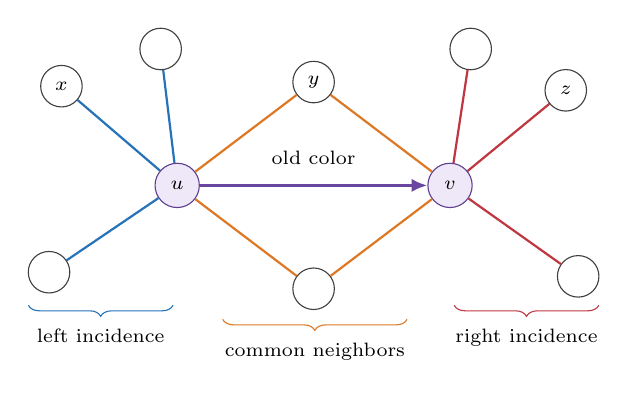
\begin{tikzpicture}[scale=1.05]
  \node[rootv] (u) at (0,0) {$u$};
  \node[rootv] (v) at (3.3,0) {$v$};
  \draw[rootedge] (u) -- (v);

  \node[vtx] (x1) at (-1.4,1.2) {$x$};
  \node[vtx] (x2) at (-1.55,-1.05) {};
  \node[vtx] (x3) at (-0.2,1.65) {};
  \draw[leftedge] (u) -- (x1);
  \draw[leftedge] (u) -- (x2);
  \draw[leftedge] (u) -- (x3);

  \node[vtx] (z1) at (4.7,1.15) {$z$};
  \node[vtx] (z2) at (4.85,-1.1) {};
  \node[vtx] (z3) at (3.55,1.65) {};
  \draw[rightedge] (v) -- (z1);
  \draw[rightedge] (v) -- (z2);
  \draw[rightedge] (v) -- (z3);

  \node[vtx] (y1) at (1.65,1.25) {$y$};
  \node[vtx] (y2) at (1.65,-1.25) {};
  \draw[triedge] (u) -- (y1);
  \draw[triedge] (v) -- (y1);
  \draw[triedge] (u) -- (y2);
  \draw[triedge] (v) -- (y2);

  \draw[decorate,decoration={brace,amplitude=4pt,mirror},leftblue]
    (-1.8,-1.45) -- (-.05,-1.45) node[midway,below=5pt,black,font=\scriptsize] {left incidence};
  \draw[decorate,decoration={brace,amplitude=4pt,mirror},triorange]
    (.55,-1.62) -- (2.78,-1.62) node[midway,below=5pt,black,font=\scriptsize] {common neighbors};
  \draw[decorate,decoration={brace,amplitude=4pt,mirror},rightred]
    (3.35,-1.45) -- (5.1,-1.45) node[midway,below=5pt,black,font=\scriptsize] {right incidence};

  \node[font=\scriptsize,align=center] at (1.65,.33) {old\ color};
\end{tikzpicture}
\caption{The EB-1WL update at an ordered edge $(u,v)$.  The purple arrow is the ordered edge being refined.  Blue edges contribute to the left-incidence multiset, red edges to the right-incidence multiset, and orange two-edge wedges through common neighbors contribute paired colors.}
\label{fig:eb-update}
\end{figure}

Let $\mathrm{eb}_G(u,v)$ denote the eventual stable color of $(u,v)$.  Since the partition of the finite set $\vecE(G)$ refines at every round, stabilization occurs after at most $|\vecE(G)|$ strict refinements.

The graph-level EB-1WL signature used in \cite{EBWL} is
\[
\Sig_{\mathrm{pair}}(G)
=
\left(|V(G)|,
\mset{\mset{\mathrm{eb}_G(u,v),\mathrm{eb}_G(v,u)}:uv\in E(G)}\right).
\]
Thus two graphs are EB-1WL-indistinguishable, written
\[
G\equiv_{\mathrm{EB\text{-}1WL}} H,
\]
if $\Sig_{\mathrm{pair}}(G)=\Sig_{\mathrm{pair}}(H)$ up to a consistent renaming of stable colors across the disjoint union $G\sqcup H$.  Equivalently, one may run the refinement on $G\sqcup H$ and compare the two induced signatures.

\begin{remark}[Graphs with isolated vertices]
The original paper assumes, for technical simplicity, that graphs have no isolated vertices.  The signature above includes $|V(G)|$, so the theorem in this manuscript extends harmlessly to graphs with isolated vertices.  Homomorphism counts from $K_1$ recover $|V(G)|$.  Connected patterns with at least one edge never map an edge to an isolated vertex, so no further modification is needed.
\end{remark}

\subsection{Computational cost and EB-GNNs}

The costly part of \eqref{eq:eb-old}--\eqref{eq:eb-right} is the common-neighbor aggregation \eqref{eq:eb-triangle}.  Using the Chiba--Nishizeki triangle-enumeration method, every triangle can be enumerated in $O(\alpha m)$ time, where $\alpha$ is the arboricity of the graph and $m=|E(G)|$ \cite{ChibaNishizeki1985}.  The EB-WL paper consequently proves that one EB-1WL iteration can be implemented in $O(m)$ space and $O(\alpha m)$ time \cite{EBWL}.  This is the computational reason EB-1WL is meant to sit between scalable 1-WL-style methods and more expensive pair-based 2-WL-style methods.

The same paper defines EB-GNNs by replacing the discrete color tuple with trainable edge features.  At layer $i$, each ordered edge $(u,v)$ carries a vector $f^{(i)}(u,v)$.  The layer computes three permutation-invariant aggregations corresponding to \eqref{eq:eb-left}, \eqref{eq:eb-triangle}, and \eqref{eq:eb-right}, combines them with the previous feature of $(u,v)$, and applies a feed-forward map.  Schematically,
\begin{align*}
A^{(i)}(u)      &\approx \sum_{x\in N(u)} \Phi_L^{(i)}\bigl(f^{(i-1)}(u,x)\bigr),\\
B^{(i)}(u,v)    &\approx \sum_{y\in N(u)\cap N(v)} \Phi_T^{(i)}\bigl(f^{(i-1)}(u,y),f^{(i-1)}(v,y)\bigr),\\
C^{(i)}(v)      &\approx \sum_{z\in N(v)} \Phi_R^{(i)}\bigl(f^{(i-1)}(v,z)\bigr),\\
 f^{(i)}(u,v)   &\approx \Psi^{(i)}\bigl(f^{(i-1)}(u,v),A^{(i)}(u),B^{(i)}(u,v),C^{(i)}(v)\bigr).
\end{align*}
The exact architecture in \cite{EBWL} uses affine maps, ReLU, and a final edge-sum readout.  The important point for this manuscript is that the neural architecture is designed to match the discrete EB-1WL refinement: the paper proves that pairs of graphs distinguishable by EB-1WL are also distinguishable by EB-GNNs, with a finite feature dimension depending on the number of edge and triangle states \cite{EBWL}.  Hence a homomorphism characterization of EB-1WL is also a clean expressivity characterization for the idealized EB-GNN family.

\section{An edge-rooted Ehrenfeucht--Fra\"iss\'e game for EB-1WL}
\label{sec:ef-game}

This section defines a finite-round game whose positions are ordered edges.  It is not the classical vertex-pebble EF game; rather, it is the exact game obtained by reading \eqref{eq:eb-old}--\eqref{eq:eb-right} as a back-and-forth condition on edge neighborhoods and triangle witnesses.

\begin{definition}[The $r$-round game $\EBEF_r$]
Let $G,H$ be finite graphs.  A position is a pair
\[
\bigl((u,v),(u',v')\bigr)\in \vecE(G)\times\vecE(H).
\]
Duplicator wins every $0$-round position.

For $r+1$ rounds, Spoiler chooses one of the following moves.  Each move may be played starting from either graph; only the $G$-to-$H$ versions are written.
\begin{enumerate}[label=\textup{(\roman*)},leftmargin=2.4em]
\item \textbf{Stay.}  The next position is again $((u,v),(u',v'))$ and $r$ rounds remain.

\item \textbf{Left incidence.}  Duplicator chooses a bijection
\[
\beta_L:N_G(u)\to N_H(u').
\]
If no such bijection exists, Duplicator loses immediately.  Spoiler chooses $x\in N_G(u)$, and the next position is
\[
\bigl((u,x),(u',\beta_L(x))\bigr).
\]

\item \textbf{Right incidence.}  Duplicator chooses a bijection
\[
\beta_R:N_G(v)\to N_H(v').
\]
Spoiler chooses $z\in N_G(v)$, and the next position is
\[
\bigl((v,z),(v',\beta_R(z))\bigr).
\]

\item \textbf{Triangle.}  Duplicator chooses a bijection
\[
\beta_T:N_G(u)\cap N_G(v)\to N_H(u')\cap N_H(v').
\]
Spoiler chooses $y\in N_G(u)\cap N_G(v)$ and then chooses one of the two incident ordered edges.  If Spoiler chooses the $u$-side, the next position is
\[
\bigl((u,y),(u',\beta_T(y))\bigr).
\]
If Spoiler chooses the $v$-side, the next position is
\[
\bigl((v,y),(v',\beta_T(y))\bigr).
\]
\end{enumerate}
Duplicator wins the $(r+1)$-round position if she has a legal response to every Spoiler move such that the resulting $r$-round position is Duplicator-winning.  The symmetric versions of the moves, where Spoiler starts in $H$ and Duplicator maps back to $G$, are included.
\end{definition}

\begin{figure}[ht]
\centering
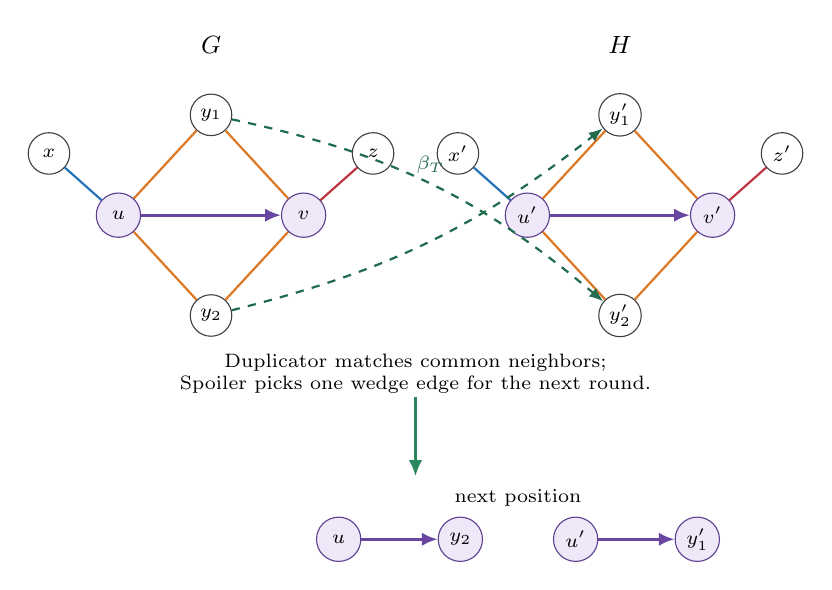
\begin{tikzpicture}[scale=.98]
  % Left graph G
  \node[font=\small] at (0,2.2) {$G$};
  \node[rootv] (gu) at (-1.2,0) {$u$};
  \node[rootv] (gv) at (1.2,0) {$v$};
  \draw[rootedge] (gu)--(gv);
  \node[vtx] (gy1) at (0,1.3) {$y_1$};
  \node[vtx] (gy2) at (0,-1.3) {$y_2$};
  \draw[triedge] (gu)--(gy1); \draw[triedge] (gv)--(gy1);
  \draw[triedge] (gu)--(gy2); \draw[triedge] (gv)--(gy2);
  \node[vtx] (gx) at (-2.1,.8) {$x$}; \draw[leftedge] (gu)--(gx);
  \node[vtx] (gz) at (2.1,.8) {$z$}; \draw[rightedge] (gv)--(gz);

  % Right graph H
  \begin{scope}[xshift=5.3cm]
  \node[font=\small] at (0,2.2) {$H$};
  \node[rootv] (hu) at (-1.2,0) {$u'$};
  \node[rootv] (hv) at (1.2,0) {$v'$};
  \draw[rootedge] (hu)--(hv);
  \node[vtx] (hy1) at (0,1.3) {$y'_1$};
  \node[vtx] (hy2) at (0,-1.3) {$y'_2$};
  \draw[triedge] (hu)--(hy1); \draw[triedge] (hv)--(hy1);
  \draw[triedge] (hu)--(hy2); \draw[triedge] (hv)--(hy2);
  \node[vtx] (hx) at (-2.1,.8) {$x'$}; \draw[leftedge] (hu)--(hx);
  \node[vtx] (hz) at (2.1,.8) {$z'$}; \draw[rightedge] (hv)--(hz);
  \end{scope}

  \draw[bij] (gy1) to[bend left=14] node[above,font=\scriptsize] {$\beta_T$} (hy2);
  \draw[bij] (gy2) to[bend right=12] (hy1);
  \node[font=\scriptsize,align=center] at (2.65,-2.05) {Duplicator matches common neighbors;\\ Spoiler picks one wedge edge for the next round.};

  % Next state mini panel
  \begin{scope}[xshift=2.65cm,yshift=-4.2cm,scale=.83]
    \node[rootv] (nu) at (-1.2,0) {$u$};
    \node[rootv] (ny) at (.7,0) {$y_2$};
    \draw[rootedge] (nu)--(ny);
    \node[rootv] (nup) at (2.5,0) {$u'$};
    \node[rootv] (nyp) at (4.4,0) {$y'_1$};
    \draw[rootedge] (nup)--(nyp);
    \node[font=\scriptsize] at (1.6,.65) {next position};
  \end{scope}
  \draw[gamearrow] (2.65,-2.35) -- (2.65,-3.38);
\end{tikzpicture}
\caption{A triangle move in the edge EF game.  Duplicator supplies a bijection between common-neighbor sets.  Spoiler picks a common neighbor and then chooses which of the two ordered wedge edges becomes the next game position.}
\label{fig:ef-triangle}
\end{figure}

\begin{theorem}[Game characterization of EB colors]
\label{thm:game-color}
For all finite graphs $G,H$, all ordered edges $(u,v)\in\vecE(G)$ and $(u',v')\in\vecE(H)$, and all $r\geq 0$,
\[
\mathrm{eb}^{(r)}_G(u,v)=\mathrm{eb}^{(r)}_H(u',v')
\]
if and only if Duplicator wins
\[
\EBEF_r\bigl(G,H;(u,v),(u',v')\bigr).
\]
\end{theorem}

\begin{proof}
The proof is by induction on $r$.

For $r=0$, every ordered edge in every graph has the same initial color.  Duplicator wins every $0$-round position by definition.

Assume the claim holds for $r$.  Consider ordered edges $(u,v)\in\vecE(G)$ and $(u',v')\in\vecE(H)$.

First suppose
\[
\mathrm{eb}^{(r+1)}_G(u,v)=\mathrm{eb}^{(r+1)}_H(u',v').
\]
By the EB update, the four components \eqref{eq:eb-old}--\eqref{eq:eb-right} agree.
The old-color components agree, so
\[
\mathrm{eb}^{(r)}_G(u,v)=\mathrm{eb}^{(r)}_H(u',v').
\]
If Spoiler plays the stay move, Duplicator keeps the same position and wins the remaining $r$ rounds by the induction hypothesis.

For a left-incidence move, equality of the left multisets gives
\[
\mset{\mathrm{eb}^{(r)}_G(u,x):x\in N_G(u)}
=
\mset{\mathrm{eb}^{(r)}_H(u',x'):x'\in N_H(u')}.
\]
Therefore Duplicator can choose a bijection $\beta_L:N_G(u)\to N_H(u')$ preserving the $r$-round EB color of every incident ordered edge:
\[
\mathrm{eb}^{(r)}_G(u,x)=\mathrm{eb}^{(r)}_H(u',\beta_L(x))
\quad\text{for all }x\in N_G(u).
\]
After Spoiler chooses $x$, the induction hypothesis gives Duplicator a winning strategy from $((u,x),(u',\beta_L(x)))$ for the remaining $r$ rounds.  The right-incidence move is identical, using equality of the right multisets.

For a triangle move, equality of the triangle multisets gives
\begin{align*}
&\mset{\bigl(\mathrm{eb}^{(r)}_G(u,y),\mathrm{eb}^{(r)}_G(v,y)\bigr):y\in N_G(u)\cap N_G(v)}\\
&\qquad=
\mset{\bigl(\mathrm{eb}^{(r)}_H(u',y'),\mathrm{eb}^{(r)}_H(v',y')\bigr):y'\in N_H(u')\cap N_H(v')}.
\end{align*}
Thus Duplicator can choose a bijection $\beta_T$ from $N_G(u)\cap N_G(v)$ to $N_H(u')\cap N_H(v')$ preserving the ordered pair of $r$-round colors.  If Spoiler chooses $y$ and then the $u$-side, then
\[
\mathrm{eb}^{(r)}_G(u,y)=\mathrm{eb}^{(r)}_H(u',\beta_T(y)),
\]
and the induction hypothesis applies.  If Spoiler chooses the $v$-side, the second coordinate of the preserved pair gives the same conclusion.  The moves starting from $H$ are symmetric.  Hence Duplicator wins $\EBEF_{r+1}$.

Conversely, suppose the $(r+1)$-round EB colors differ.  Since a color is the full tuple in \eqref{eq:eb-old}--\eqref{eq:eb-right}, at least one component differs.

If the old-color component differs, Spoiler plays stay.  The resulting $r$-round position has different $r$-round colors, so Spoiler wins by the induction hypothesis.

If the left multiset differs, then no bijection $\beta_L:N_G(u)\to N_H(u')$ can preserve all $r$-round colors.  Spoiler plays a left-incidence move from the side witnessing the multiset difference.  Whatever bijection Duplicator chooses, there is some selected neighbor whose matched ordered edge has a different $r$-round color.  Spoiler chooses that neighbor and wins by the induction hypothesis.  The right-incidence case is identical.

Finally, if the triangle-pair multiset differs, then no bijection between the common-neighbor sets can preserve every ordered pair of $r$-round colors.  Spoiler plays a triangle move from a side witnessing the difference.  After Duplicator chooses $\beta_T$, Spoiler selects a common neighbor $y$ for which the pair
\[
\bigl(\mathrm{eb}^{(r)}(u,y),\mathrm{eb}^{(r)}(v,y)\bigr)
\]
is not matched correctly.  At least one coordinate of the pair differs, and Spoiler chooses the corresponding wedge edge.  The induction hypothesis again gives a win for the remaining $r$ rounds.

This proves the equivalence for $r+1$ and completes the induction.
\end{proof}

\section{Rooted chordal patterns}
\label{sec:rooted-patterns}

The homomorphism side of the proof uses patterns with a distinguished ordered root edge.

\begin{definition}[Rooted oriented-edge pattern]
A rooted oriented-edge pattern is a pair $(P,\rho)$ where $P$ is a finite graph and $\rho=(a,b)\in\vecE(P)$ is an ordered edge.  For $G$ a host graph and $(u,v)\in\vecE(G)$, define
\[
h_{P,\rho}^G(u,v)
=
\#\{\varphi:P\to G:\varphi(a)=u,\ \varphi(b)=v\}.
\]
When $\rho$ is clear, write $h_P^G(u,v)$.
\end{definition}

We now define a class $\cR$ of rooted patterns.  The operations are chosen so that their rooted homomorphism counts are exactly the algebraic operations appearing in the EB update.

\begin{definition}[The rooted pattern class $\cR$]
The class $\cR$ is the smallest class of rooted oriented-edge patterns closed under the following operations.

\begin{enumerate}[label=\textup{(\Alph*)},leftmargin=2.4em]
\item \textbf{Base edge.}  The single edge $K_2$ rooted in either orientation is in $\cR$.

\item \textbf{Root-edge product.}  If $(P,(a,b))$ and $(Q,(c,d))$ are in $\cR$, their product $P\odot Q$ is obtained from the disjoint union of $P$ and $Q$ by identifying $a$ with $c$ and $b$ with $d$.  The root is the identified ordered edge.

\item \textbf{Left extension.}  If $(P,(a,b))\in\cR$, define $L(P)$ by adding a new vertex $s$ adjacent to $a$ and declaring the new root to be $(a,s)$.  The old root edge $(a,b)$ remains inside the pattern.

\item \textbf{Right extension.}  If $(P,(a,b))\in\cR$, define $R(P)$ by adding a new vertex $r$ adjacent to $a$ and declaring the new root to be $(r,a)$.  The old root edge $(a,b)$ remains inside the pattern.

\item \textbf{Triangle extension.}  If $(P,(a,b))$ and $(Q,(c,d))$ are in $\cR$, define $T(P,Q)$ as follows.  Start with a triangle on vertices $r,s,w$ and root edge $(r,s)$.  Glue the root $(a,b)$ of $P$ to the ordered edge $(r,w)$ and glue the root $(c,d)$ of $Q$ to the ordered edge $(s,w)$.  The root of the resulting graph is $(r,s)$.
\end{enumerate}
\end{definition}

\begin{figure}[ht]
\centering
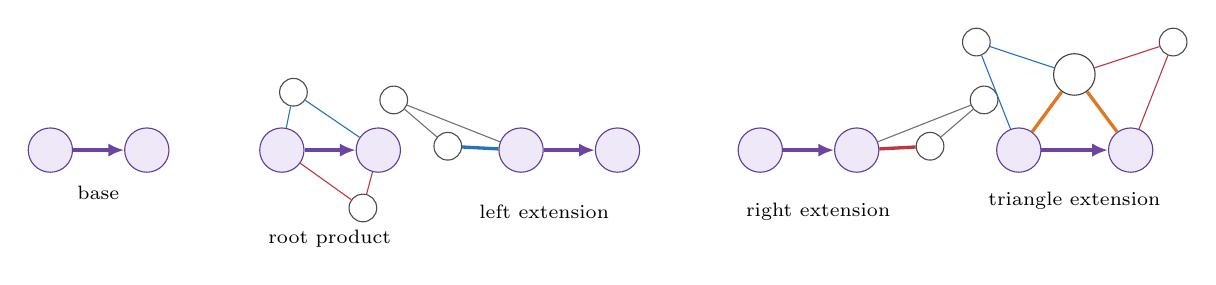
\begin{tikzpicture}[scale=.98]
  % Base
  \begin{scope}[xshift=0cm]
    \node[rootv] (a) at (0,0) {};
    \node[rootv] (b) at (1.25,0) {};
    \draw[rootedge] (a)--(b);
    \node[font=\scriptsize] at (.62,-.55) {base};
  \end{scope}

  % Product
  \begin{scope}[xshift=3.0cm]
    \node[rootv] (p1) at (0,0) {};
    \node[rootv] (p2) at (1.25,0) {};
    \draw[rootedge] (p1)--(p2);
    \node[tinyv] (p3) at (.15,.75) {};
    \node[tinyv] (p4) at (1.05,-.75) {};
    \draw[leftblue] (p1)--(p3)--(p2);
    \draw[rightred] (p1)--(p4)--(p2);
    \node[font=\scriptsize] at (.62,-1.15) {root product};
  \end{scope}

  % Left
  \begin{scope}[xshift=6.1cm]
    \node[rootv] (l1) at (0,0) {};
    \node[rootv] (l2) at (1.25,0) {};
    \draw[rootedge] (l1)--(l2);
    \node[tinyv] (lold) at (-.95,.05) {};
    \node[tinyv] (lint) at (-1.65,.65) {};
    \draw[leftedge,very thick] (l1)--(lold);
    \draw[black!55] (lold)--(lint)--(l1);
    \node[font=\scriptsize] at (.3,-.8) {left extension};
  \end{scope}

  % Right
  \begin{scope}[xshift=9.2cm]
    \node[rootv] (r1) at (0,0) {};
    \node[rootv] (r2) at (1.25,0) {};
    \draw[rootedge] (r1)--(r2);
    \node[tinyv] (rold) at (2.2,.05) {};
    \node[tinyv] (rint) at (2.9,.65) {};
    \draw[rightedge,very thick] (r2)--(rold);
    \draw[black!55] (rold)--(rint)--(r2);
    \node[font=\scriptsize] at (.75,-.8) {right extension};
  \end{scope}

  % Triangle
  \begin{scope}[xshift=12.55cm]
    \node[rootv] (t1) at (0,0) {};
    \node[rootv] (t2) at (1.45,0) {};
    \node[vtx] (tw) at (.72,.98) {};
    \draw[rootedge] (t1)--(t2);
    \draw[triedge,very thick] (t1)--(tw)--(t2);
    \node[tinyv] (tp) at (-.55,1.4) {};
    \node[tinyv] (tq) at (2.0,1.4) {};
    \draw[leftblue] (t1)--(tp)--(tw);
    \draw[rightred] (t2)--(tq)--(tw);
    \node[font=\scriptsize] at (.72,-.65) {triangle extension};
  \end{scope}
\end{tikzpicture}
\caption{The generators of the rooted pattern calculus.  Purple arrows mark the current root edge.  Blue and red subpatterns attach to the left and right endpoints; the triangle extension shares one witness vertex across both sides, mirroring the EB common-neighbor update.}
\label{fig:pattern-ops}
\end{figure}

The following identities are immediate from the definitions.  They are the reason these operations are exactly the right ones.

\begin{lemma}[Rooted count identities]
\label{lem:rooted-identities}
For every host graph $G$ and ordered edge $(u,v)\in\vecE(G)$:
\begin{align*}
h_{K_2}^G(u,v)&=1,\\
h_{P\odot Q}^G(u,v)&=h_P^G(u,v)\,h_Q^G(u,v),\\
h_{L(P)}^G(u,v)&=\sum_{x\in N_G(u)} h_P^G(u,x),\\
h_{R(P)}^G(u,v)&=\sum_{z\in N_G(v)} h_P^G(v,z),\\
h_{T(P,Q)}^G(u,v)&=\sum_{y\in N_G(u)\cap N_G(v)} h_P^G(u,y)\,h_Q^G(v,y).
\end{align*}
\end{lemma}

\begin{proof}
The base identity is clear because a homomorphism from the rooted edge $K_2$ to $G$ sending the root to $(u,v)$ is unique.

For $P\odot Q$, a rooted homomorphism of the glued graph to $G$ with root $(u,v)$ is exactly a pair consisting of a rooted homomorphism $P\to G$ with root $(u,v)$ and a rooted homomorphism $Q\to G$ with root $(u,v)$.  These choices are independent after the root vertices are fixed, giving the product.

For $L(P)$, the new root is $(a,s)$ while the old root of $P$ is $(a,b)$.  If $a$ maps to $u$ and $s$ maps to $v$, then the old root vertex $b$ may map to any neighbor $x\in N_G(u)$, and the number of extensions inside $P$ is $h_P^G(u,x)$.  Summing over $x$ gives the formula.  The proof for $R(P)$ is the same with the roles of the endpoints shifted.

For $T(P,Q)$, a rooted homomorphism with $r\mapsto u$ and $s\mapsto v$ sends the triangle witness vertex $w$ to a common neighbor $y\in N_G(u)\cap N_G(v)$.  After $y$ is chosen, the copy of $P$ rooted at $(r,w)$ contributes $h_P^G(u,y)$ choices and the copy of $Q$ rooted at $(s,w)$ contributes $h_Q^G(v,y)$ choices.  Summing over $y$ gives the identity.
\end{proof}

\begin{lemma}[Patterns in $\cR$ are chordal of treewidth at most two]
\label{lem:R-chordal}
If $(P,\rho)\in\cR$, then $P$ is chordal and $\tw(P)\leq 2$.
\end{lemma}

\begin{proof}
It is enough to show that every operation preserves chordality and maximum clique size at most three.  The base edge has this property.

The root-edge product is a clique-sum along a clique of size two.  Clique-sums of chordal graphs along cliques are chordal, and no clique larger than the cliques already present is created.  Thus the maximum clique size remains at most three.

The left and right extensions add one new vertex adjacent to exactly one old vertex.  The new vertex is simplicial and creates only a clique of size two.  Chordality and the maximum-clique bound are preserved.

The triangle extension starts with a triangle, then glues $P$ along the clique $\{r,w\}$ and $Q$ along the clique $\{s,w\}$.  Again these are clique-sums along cliques.  The only new maximal clique introduced by the central gadget is the triangle $\{r,s,w\}$.  Hence the resulting graph is chordal and has maximum clique size at most three.  Since chordal graphs have treewidth equal to maximum clique size minus one, every graph produced has treewidth at most two.
\end{proof}

We also need the converse generation fact in order to give a self-contained proof of the original lower-bound theorem.

\begin{lemma}[Rooted generation of connected chordal treewidth-two graphs]
\label{lem:R-generates}
Let $F$ be a connected chordal graph with $\tw(F)\leq 2$, and suppose $F$ has at least one edge.  For every oriented edge $\rho=(a,b)\in\vecE(F)$, the rooted graph $(F,\rho)$ belongs to $\cR$.
\end{lemma}

\begin{proof}
We prove the claim by induction on the number of maximal cliques of $F$.  Since $F$ is chordal and has treewidth at most two, every maximal clique has size one, two, or three.  Because $F$ is connected and has an edge, the relevant maximal cliques have size two or three, except for the one-vertex graph which is excluded.

If $F$ has exactly one maximal clique, then $F$ is either $K_2$ or $K_3$.  The rooted $K_2$ is a base pattern.  A rooted triangle with root $(a,b)$ is $T(K_2,K_2)$: the two base edges are glued to $(a,w)$ and $(b,w)$ around the central triangle $(a,b,w)$.

Now assume the claim for graphs with fewer maximal cliques.  Fix the oriented root edge $(a,b)$.  Choose a clique tree $\mathcal{T}$ of $F$.  If the root edge $\{a,b\}$ is not itself a maximal clique, add an auxiliary root bag $B_0=\{a,b\}$ and connect it to one maximal clique containing $\{a,b\}$.  If several maximal cliques contain $\{a,b\}$, choose the clique tree so that they are all adjacent to $B_0$; this is possible because the bags containing any fixed clique form a connected subtree, and replacing that subtree by a star centered at $B_0$ preserves the clique-tree running-intersection property.  Root the resulting bag tree at $B_0$.

Delete $B_0$ from this rooted tree.  Each connected component $C$ of the remaining tree attaches to $B_0$ through a separator
\[
S_C\subseteq \{a,b\}.
\]
Since $F$ is connected and every non-root component contains a vertex outside $\{a,b\}$, the separator is one of $\{a\}$, $\{b\}$, or $\{a,b\}$.  The subgraphs induced by distinct components intersect only in the root vertices $a,b$.  Thus the rooted graph $(F,(a,b))$ is obtained by root-edge products of the root edge $K_2$ with one rooted contribution for each component $C$.  It remains to show that each component contribution is produced by a left extension, a right extension, or a triangle extension applied to smaller rooted chordal graphs.

First suppose $S_C=\{a\}$.  Let $F_C$ be the subgraph induced by $a$ together with all vertices appearing in bags of $C$.  Then $F_C$ is connected, chordal, and has treewidth at most two.  Since $C$ attaches through $a$, there is some neighbor $x$ of $a$ in $F_C$.  Choose such an $x$ from the bag of $C$ adjacent to $B_0$.  The rooted graph $(F_C,(a,x))$ has fewer maximal cliques than $F$ unless $F$ is just the edge $ax$ plus the root edge $ab$, and that exceptional case is also covered by the base pattern.  By induction, $(F_C,(a,x))\in\cR$.  Applying $L$ adds the root vertex $b$ adjacent to $a$ and gives precisely the contribution of this component together with the root edge $ab$.

The case $S_C=\{b\}$ is symmetric.  Choose a neighbor $z$ of $b$ in the component subgraph $F_C$; by induction $(F_C,(b,z))\in\cR$, and applying the right-extension operation, with the new root oriented as $(a,b)$, gives the required contribution.

Now suppose $S_C=\{a,b\}$.  The bag of $C$ adjacent to $B_0$ must be a triangle $\{a,b,y\}$ for some vertex $y\notin\{a,b\}$.  By the choice of the clique tree, no descendant component below this triangle attaches again through the root separator $\{a,b\}$; any remaining descendant attaches through one of the cliques $\{a,y\}$, $\{b,y\}$, $\{a\}$, $\{b\}$, or $\{y\}$.  Partition those descendant branches into two groups: put every branch whose separator is contained in $\{a,y\}$ into the left group, and put every branch whose separator is contained in $\{b,y\}$ into the right group; branches attached only through $\{y\}$ may be assigned arbitrarily, say to the left group.  Let $F_L$ be the subgraph induced by $a,y$ and all vertices in the left group, and let $F_R$ be the subgraph induced by $b,y$ and all vertices in the right group.  Both are connected chordal graphs of treewidth at most two with fewer maximal cliques than $F$, unless one is just a single edge.  By induction and the base case,
\[
(F_L,(a,y))\in\cR,
\qquad
(F_R,(b,y))\in\cR.
\]
The triangle extension $T(F_L,F_R)$ produces exactly the triangle $a b y$ together with the two assigned families of descendants, rooted at $(a,b)$.

Taking the root-edge product over all component contributions reconstructs $(F,(a,b))$.  Since $\cR$ is closed under root-edge product, $(F,(a,b))\in\cR$.
\end{proof}

\begin{figure}[ht]
\centering
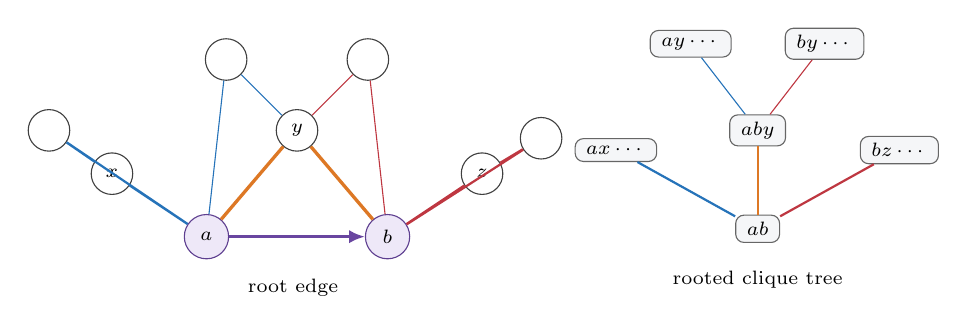
\begin{tikzpicture}[scale=1]
  % graph side
  \node[rootv] (a) at (0,0) {$a$};
  \node[rootv] (b) at (2.3,0) {$b$};
  \draw[rootedge] (a)--(b);
  \node[vtx] (x) at (-1.2,.8) {$x$};
  \node[vtx] (x2) at (-2,1.35) {};
  \draw[leftedge] (a)--(x)--(x2)--(a);
  \node[vtx] (z) at (3.5,.8) {$z$};
  \node[vtx] (z2) at (4.25,1.25) {};
  \draw[rightedge] (b)--(z)--(z2)--(b);
  \node[vtx] (y) at (1.15,1.35) {$y$};
  \draw[triedge,very thick] (a)--(y)--(b);
  \node[vtx] (p) at (.25,2.25) {};
  \node[vtx] (q) at (2.05,2.25) {};
  \draw[leftblue] (a)--(p)--(y);
  \draw[rightred] (b)--(q)--(y);
  \node[font=\scriptsize] at (1.1,-.65) {root edge};

  % clique tree side
  \begin{scope}[xshift=7.0cm,yshift=.1cm]
    \node[bag] (ab) at (0,0) {$ab$};
    \node[bag] (ax) at (-1.8,1.0) {$ax\cdots$};
    \node[bag] (aby) at (0,1.25) {$aby$};
    \node[bag] (bz) at (1.8,1.0) {$bz\cdots$};
    \node[bag] (ay) at (-.85,2.35) {$ay\cdots$};
    \node[bag] (by) at (.85,2.35) {$by\cdots$};
    \draw[leftedge] (ab)--(ax);
    \draw[triedge] (ab)--(aby);
    \draw[rightedge] (ab)--(bz);
    \draw[leftblue] (aby)--(ay);
    \draw[rightred] (aby)--(by);
    \node[font=\scriptsize] at (0,-.65) {rooted clique tree};
  \end{scope}
\end{tikzpicture}
\caption{The rooted generation lemma.  Around a root edge $ab$, every clique-tree branch attaches through $a$, through $b$, or through the edge $ab$ via a triangle $aby$.  These are exactly left extensions, right extensions, and triangle extensions, glued together by root-edge product.}
\label{fig:clique-tree-generation}
\end{figure}

\section{The original homomorphism lower bound, proved from the calculus}
\label{sec:original-direction}

The original EB-WL paper proves \Cref{thm:original-lower-bound}.  We include a proof because it also explains why the pattern operations are the correct dual objects to EB-1WL.

\begin{lemma}[Rooted counts are determined by sufficiently deep EB colors]
\label{lem:counts-determined-by-color}
For every rooted pattern $(P,\rho)\in\cR$, there is a round $t(P)\geq 0$ and a function
\[
\eta_P:\{\text{EB colors appearing at round }t(P)\}\to\N
\]
such that for every graph $G$ and every ordered edge $(u,v)\in\vecE(G)$,
\[
h_P^G(u,v)=\eta_P\bigl(\mathrm{eb}^{(t(P))}_G(u,v)\bigr).
\]
\end{lemma}

\begin{proof}
Induct over the construction of $P$.

For the base edge $K_2$, take $t(P)=0$ and $\eta_P\equiv 1$.

For a root-edge product $P\odot Q$, choose $t=\max(t(P),t(Q))$.  EB colors refine with time, so the round-$t$ color determines the round-$t(P)$ color and the round-$t(Q)$ color.  Hence it determines both $h_P$ and $h_Q$, and by \Cref{lem:rooted-identities} it determines $h_{P\odot Q}=h_P h_Q$.

For a left extension $L(P)$, let $t=t(P)+1$.  The round-$t$ EB color of $(u,v)$ contains the left-incidence multiset
\[
\mset{\mathrm{eb}^{(t(P))}_G(u,x):x\in N_G(u)}.
\]
By the induction hypothesis, each color in this multiset determines $h_P^G(u,x)$.  Therefore the multiset determines
\[
\sum_{x\in N_G(u)}h_P^G(u,x)=h_{L(P)}^G(u,v).
\]
The right extension is identical, using the right-incidence multiset.

For a triangle extension $T(P,Q)$, take $t=1+\max(t(P),t(Q))$.  The round-$t$ color of $(u,v)$ determines the multiset of pairs
\[
\mset{\bigl(\mathrm{eb}^{(t-1)}_G(u,y),\mathrm{eb}^{(t-1)}_G(v,y)\bigr):y\in N_G(u)\cap N_G(v)}.
\]
Since round-$(t-1)$ colors determine the relevant earlier colors for both $P$ and $Q$, this paired multiset determines
\[
\sum_{y\in N_G(u)\cap N_G(v)}h_P^G(u,y)h_Q^G(v,y)
=h_{T(P,Q)}^G(u,v).
\]
Thus the claim holds for every operation.
\end{proof}

\begin{theorem}[Self-contained proof of the original direction]
\label{thm:original-direction-self-contained}
If $G\equiv_{\mathrm{EB\text{-}1WL}}H$, then
\[
\hom(F,G)=\hom(F,H)
\qquad\text{for every }F\in\cC_2^\triangle.
\]
Equivalently, if some $F\in\cC_2^\triangle$ has $\hom(F,G)\neq\hom(F,H)$, then EB-1WL distinguishes $G,H$.
\end{theorem}

\begin{proof}
Assume $G\equiv_{\mathrm{EB\text{-}1WL}}H$ under the pair signature $\Sig_{\mathrm{pair}}$.  Then $|V(G)|=|V(H)|$, and the stable multiset of unordered pairs of opposite ordered-edge colors is the same in $G$ and $H$.  In particular, for each stable color $c$, the number of ordered edges of color $c$ is the same in $G$ and $H$: it is obtained by summing the multiplicities of all unordered edge-pair types containing $c$, with multiplicity two for the type $\mset{c,c}$.

Let $F\in\cC_2^\triangle$.  Since homomorphism counts multiply over connected components,
\[
\hom(F,G)=\prod_{C\in\mathrm{cc}(F)}\hom(C,G),
\]
it suffices to handle connected $F$.

If $F=K_1$, then $\hom(F,G)=|V(G)|=|V(H)|=\hom(F,H)$.

Otherwise $F$ is connected and has at least one edge.  Choose an oriented root edge $\rho=(a,b)\in\vecE(F)$.  By \Cref{lem:R-generates}, $(F,\rho)\in\cR$.  By \Cref{lem:counts-determined-by-color}, for all ordered host edges $(u,v)$,
\[
h_{F,\rho}^G(u,v)=\eta\bigl(\mathrm{eb}_G(u,v)\bigr)
\]
for a function $\eta$ of the stable EB color.  Therefore
\[
\hom(F,G)=\sum_{(u,v)\in\vecE(G)} h_{F,\rho}^G(u,v)
=\sum_{(u,v)\in\vecE(G)}\eta\bigl(\mathrm{eb}_G(u,v)\bigr).
\]
The last expression depends only on the stable ordered-edge color histogram, which is determined by $\Sig_{\mathrm{pair}}(G)$.  Since $\Sig_{\mathrm{pair}}(G)=\Sig_{\mathrm{pair}}(H)$, the same expression has the same value for $H$.  Hence $\hom(F,G)=\hom(F,H)$.
\end{proof}

\section{The converse: EB color differences produce chordal homomorphism witnesses}
\label{sec:converse}

We now prove the new direction.  The proof is algebraic, but each algebraic operation has an EF-game interpretation: it records a finite menu of Spoiler tests and compiles them into rooted homomorphism patterns.

Fix two graphs $G,H$ and run EB-1WL on the disjoint union $G\sqcup H$, so color names are globally comparable.  Let
\[
\Omega=\vecE(G)\sqcup \vecE(H).
\]
Every rooted pattern $P\in\cR$ defines a function $h_P:\Omega\to\N$ by using $h_P^G$ on ordered edges of $G$ and $h_P^H$ on ordered edges of $H$.

Let $\cA$ be the $\Q$-linear span of all such rooted count functions:
\[
\cA=\operatorname{span}_{\Q}\{h_P:P\in\cR\}\subseteq \Q^\Omega.
\]
By the root-edge product identity in \Cref{lem:rooted-identities}, $\cA$ is closed under pointwise multiplication.  Indeed, if $h_P,h_Q\in\cA$, then $h_Ph_Q=h_{P\odot Q}\in\cA$, and bilinearity extends this to all rational linear combinations.

For each round $t$, let $\Pi_t$ be the partition of $\Omega$ into round-$t$ EB color classes.  For $C\in\Pi_t$, let $\mathbf{1}_C:\Omega\to\{0,1\}$ be its indicator function.

\begin{lemma}[Finite-round color classes lie in the rooted-count algebra]
\label{lem:indicator-span}
For every $t\geq 0$ and every color class $C\in\Pi_t$,
\[
\mathbf{1}_C\in\cA.
\]
Equivalently, there exist patterns $P_1,\ldots,P_m\in\cR$ and rational coefficients $\alpha_1,\ldots,\alpha_m$ such that
\[
\mathbf{1}_C(e)=\sum_{i=1}^m\alpha_i h_{P_i}(e)
\qquad\text{for every }e\in\Omega.
\]
\end{lemma}

\begin{proof}
We induct on $t$.

For $t=0$, all ordered edges have the same color.  The unique indicator is the constant function $1$, which is $h_{K_2}$, so it lies in $\cA$.

Assume the claim for round $t$.  We show it for round $t+1$.  A round-$(t+1)$ color class is determined by the following finite list of integer-valued functions on $\Omega$.

For an ordered edge $e=(u,v)$, first include the old round-$t$ color.  It is enough to include all old indicators $\mathbf{1}_D(e)$ for $D\in\Pi_t$, and these lie in $\cA$ by induction.

Next, for every old color class $D\in\Pi_t$, define the left and right neighbor-count functions
\begin{align*}
L_D(u,v)&=\sum_{x\in N(u)}\mathbf{1}_D(u,x),\\
R_D(u,v)&=\sum_{z\in N(v)}\mathbf{1}_D(v,z).
\end{align*}
By induction, write $\mathbf{1}_D=\sum_i\alpha_i h_{P_i}$.  Then
\[
L_D(u,v)=\sum_i\alpha_i\sum_{x\in N(u)}h_{P_i}(u,x)
=\sum_i\alpha_i h_{L(P_i)}(u,v),
\]
so $L_D\in\cA$.  Similarly $R_D\in\cA$.

Finally, for old color classes $D_1,D_2\in\Pi_t$, define the triangle-pair count
\[
T_{D_1,D_2}(u,v)
=\sum_{y\in N(u)\cap N(v)}\mathbf{1}_{D_1}(u,y)\mathbf{1}_{D_2}(v,y).
\]
Using the induction hypothesis, expand
\[
\mathbf{1}_{D_1}=\sum_i\alpha_i h_{P_i},
\qquad
\mathbf{1}_{D_2}=\sum_j\beta_j h_{Q_j}.
\]
Then
\begin{align*}
T_{D_1,D_2}(u,v)
&=\sum_{y\in N(u)\cap N(v)}
\left(\sum_i\alpha_i h_{P_i}(u,y)\right)
\left(\sum_j\beta_j h_{Q_j}(v,y)\right)\\
&=\sum_{i,j}\alpha_i\beta_j
\sum_{y\in N(u)\cap N(v)} h_{P_i}(u,y)h_{Q_j}(v,y)\\
&=\sum_{i,j}\alpha_i\beta_j h_{T(P_i,Q_j)}(u,v).
\end{align*}
Thus every triangle-pair count lies in $\cA$.

Let $F_1,\ldots,F_s\in\cA$ be the complete finite list of coordinate functions just described: old-color indicators, all left counts, all right counts, and all triangle-pair counts.  A round-$(t+1)$ color class $C$ is a fiber of the map
\[
e\longmapsto (F_1(e),\ldots,F_s(e))
\]
on the finite set $\Omega$.  Let the fiber value for $C$ be $(a_1,\ldots,a_s)$.  For each coordinate $j$, let
\[
S_j=\{F_j(e):e\in\Omega\}
\]
be its finite set of values.  Define the one-variable polynomial
\[
p_j(X)=\prod_{b\in S_j\setminus\{a_j\}}\frac{X-b}{a_j-b},
\]
with the convention $p_j(X)=1$ if $S_j=\{a_j\}$.  Then $p_j(F_j(e))=1$ exactly when $F_j(e)=a_j$, and $0$ otherwise.  Hence
\[
\mathbf{1}_C(e)=\prod_{j=1}^s p_j(F_j(e))
\qquad\text{for every }e\in\Omega.
\]
Because $\cA$ contains all $F_j$, contains the constant function $1$, and is closed under rational linear combinations and pointwise multiplication, this product belongs to $\cA$.  Therefore $\mathbf{1}_C\in\cA$.
\end{proof}

\begin{figure}[ht]
\centering
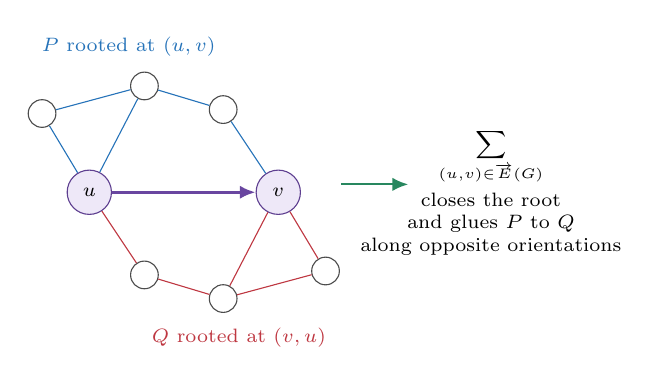
\begin{tikzpicture}[scale=1]
  % Rooted P above edge
  \node[rootv] (u) at (0,0) {$u$};
  \node[rootv] (v) at (2.4,0) {$v$};
  \draw[rootedge] (u)--(v);

  \node[tinyv] (p1) at (-.6,1.0) {};
  \node[tinyv] (p2) at (.7,1.35) {};
  \node[tinyv] (p3) at (1.7,1.05) {};
  \draw[leftblue] (u)--(p1)--(p2)--(u);
  \draw[leftblue] (p2)--(p3)--(v);
  \node[font=\scriptsize,leftblue] at (.5,1.85) {$P$ rooted at $(u,v)$};

  % Q below reversed
  \node[tinyv] (q1) at (3.0,-1.0) {};
  \node[tinyv] (q2) at (1.7,-1.35) {};
  \node[tinyv] (q3) at (.7,-1.05) {};
  \draw[rightred] (v)--(q1)--(q2)--(v);
  \draw[rightred] (q2)--(q3)--(u);
  \node[font=\scriptsize,rightred] at (1.9,-1.85) {$Q$ rooted at $(v,u)$};

  \node[font=\scriptsize,align=center] at (5.1,0) {$\displaystyle\sum_{(u,v)\in\vecE(G)}$\\[2pt]
  closes the root\\ and glues $P$ to $Q$\\ along opposite orientations};
  \draw[gamearrow] (3.2,.1) -- (4.05,.1);
\end{tikzpicture}
\caption{Closing a graph-level edge-signature difference.  The term $h_P(u,v)h_Q(v,u)$ is the rooted count of two patterns glued along the same host edge in opposite orientations.  Summing over ordered host edges gives an ordinary unrooted homomorphism count.}
\label{fig:closing-root}
\end{figure}

\begin{theorem}[Converse to the EB-WL homomorphism lower bound]
\label{thm:converse}
If $G,H$ are distinguishable by EB-1WL under the pair signature $\Sig_{\mathrm{pair}}$, then there exists $F\in\cC_2^\triangle$ such that
\[
\hom(F,G)\neq\hom(F,H).
\]
\end{theorem}

\begin{proof}
Run EB-1WL to stabilization on the disjoint union $G\sqcup H$, and let $\Pi$ be the stable partition of $\Omega=\vecE(G)\sqcup\vecE(H)$.

If $|V(G)|\neq |V(H)|$, then $F=K_1$ separates the graphs because
\[
\hom(K_1,G)=|V(G)|\neq |V(H)|=\hom(K_1,H).
\]
So assume $|V(G)|=|V(H)|$ and the edge-pair part of $\Sig_{\mathrm{pair}}$ differs.

Then there exist stable colors $c,d\in\Pi$ such that the number of undirected edges whose two oriented colors form the unordered pair $\mset{c,d}$ differs between $G$ and $H$.  Define
\[
S_{c,d}(G)=\sum_{(u,v)\in\vecE(G)}\mathbf{1}_c(u,v)\mathbf{1}_d(v,u),
\]
and define $S_{c,d}(H)$ analogously.  If $c\neq d$, then $S_{c,d}(G)$ is exactly the number of undirected edges of pair type $\mset{c,d}$.  If $c=d$, then $S_{c,c}(G)$ is twice the number of undirected edges of pair type $\mset{c,c}$.  Hence the pair-signature difference gives colors $c,d$ with
\[
S_{c,d}(G)\neq S_{c,d}(H).
\]

By \Cref{lem:indicator-span}, there are rooted patterns $P_1,\ldots,P_m,Q_1,\ldots,Q_n\in\cR$ and rational coefficients $\alpha_i,\beta_j$ such that
\[
\mathbf{1}_c(u,v)=\sum_i\alpha_i h_{P_i}^G(u,v),
\qquad
\mathbf{1}_d(v,u)=\sum_j\beta_j h_{Q_j}^G(v,u)
\]
for every ordered edge $(u,v)$ of $G$, and the same identities hold in $H$ because they were constructed on the disjoint union.

Therefore
\begin{align*}
S_{c,d}(G)
&=\sum_{(u,v)\in\vecE(G)}
\left(\sum_i\alpha_i h_{P_i}^G(u,v)\right)
\left(\sum_j\beta_j h_{Q_j}^G(v,u)\right)\\
&=\sum_{i,j}\alpha_i\beta_j
\sum_{(u,v)\in\vecE(G)}h_{P_i}^G(u,v)h_{Q_j}^G(v,u).
\end{align*}
For each pair $(i,j)$, let $F_{ij}$ be the unrooted graph obtained by gluing the root edge of $P_i$ to the reversed root edge of $Q_j$.  Explicitly, if $P_i$ is rooted at $(a_i,b_i)$ and $Q_j$ is rooted at $(c_j,d_j)$, identify
\[
a_i=d_j,
\qquad
b_i=c_j.
\]
Then
\[
\sum_{(u,v)\in\vecE(G)}h_{P_i}^G(u,v)h_{Q_j}^G(v,u)=\hom(F_{ij},G).
\]
Indeed, a homomorphism $F_{ij}\to G$ chooses the image $(u,v)$ of the glued oriented root edge and then independently chooses a rooted homomorphism from $P_i$ to $G$ with root $(u,v)$ and a rooted homomorphism from $Q_j$ to $G$ with root $(v,u)$.

By \Cref{lem:R-chordal}, $P_i$ and $Q_j$ are chordal of treewidth at most two, and gluing them along an edge is a clique-sum.  Thus every $F_{ij}$ is chordal of treewidth at most two.

The same expansion holds for $H$, so
\[
S_{c,d}(G)-S_{c,d}(H)
=\sum_{i,j}\alpha_i\beta_j
\bigl(\hom(F_{ij},G)-\hom(F_{ij},H)\bigr).
\]
The left-hand side is nonzero.  Therefore at least one summand on the right has
\[
\hom(F_{ij},G)\neq \hom(F_{ij},H).
\]
This $F_{ij}$ is the required chordal treewidth-two witness.
\end{proof}

\begin{corollary}[Main equivalence]
\label{cor:main}
For finite simple graphs $G,H$,
\[
G\equiv_{\mathrm{EB\text{-}1WL}}H
\quad\Longleftrightarrow\quad
\hom(F,G)=\hom(F,H)\quad\text{for all }F\in\cC_2^\triangle.
\]
\end{corollary}

\begin{proof}
The forward implication is \Cref{thm:original-direction-self-contained}; the reverse implication is the contrapositive of \Cref{thm:converse}.
\end{proof}

\section{How the EF game appears inside the homomorphism proof}
\label{sec:ef-inside}

The proof above can be read directly as an EF-to-homomorphism compiler.

Suppose Spoiler wins the $r$-round edge game from an ordered edge $e\in\vecE(G)$ against every candidate edge $f\in\vecE(H)$ of some color class.  By \Cref{thm:game-color}, this means that the round-$r$ EB color of $e$ is separated from those candidates.  \Cref{lem:indicator-span} says that the indicator of that winning color class is a rational linear combination of rooted counts.  The induction in \Cref{lem:indicator-span} follows Spoiler's move types:
\begin{itemize}[leftmargin=2.2em]
\item the stay move keeps the old rooted pattern;
\item the left-incidence move adds a new root edge at the left endpoint;
\item the right-incidence move adds a new root edge at the right endpoint;
\item the triangle move adds a common witness vertex and glues two rooted subpatterns along the two wedge edges.
\end{itemize}
Thus the finite EF strategy tree does not produce an arbitrary bounded-treewidth pattern; it produces a pattern assembled by clique-sums of edges and triangles.  That is exactly why the witness class is chordal treewidth two, rather than all treewidth-two graphs.

\begin{figure}[ht]
\centering
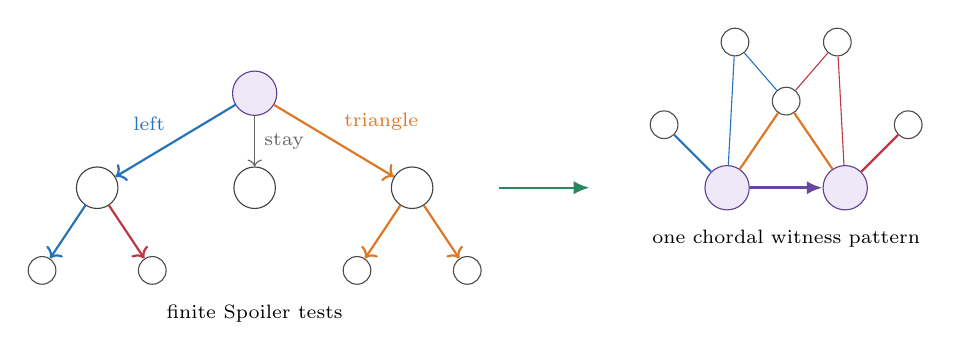
\begin{tikzpicture}[scale=1]
  % game decision tree
  \node[rootv] (root) at (0,0) {};
  \node[vtx] (l) at (-2,-1.2) {};
  \node[vtx] (r) at (0,-1.2) {};
  \node[vtx] (t) at (2,-1.2) {};
  \draw[leftedge,->] (root)--(l) node[midway,above left,font=\scriptsize] {left};
  \draw[black!60,->] (root)--(r) node[midway,right,font=\scriptsize] {stay};
  \draw[triedge,->] (root)--(t) node[midway,above right,font=\scriptsize] {triangle};
  \node[tinyv] (ll) at (-2.7,-2.25) {}; \node[tinyv] (lr) at (-1.3,-2.25) {};
  \draw[leftedge,->] (l)--(ll); \draw[rightedge,->] (l)--(lr);
  \node[tinyv] (tl) at (1.3,-2.25) {}; \node[tinyv] (tr) at (2.7,-2.25) {};
  \draw[triedge,->] (t)--(tl); \draw[triedge,->] (t)--(tr);
  \node[font=\scriptsize] at (0,-2.8) {finite Spoiler tests};

  \draw[gamearrow] (3.1,-1.2)--(4.25,-1.2);

  % pattern assembled
  \begin{scope}[xshift=6.0cm,yshift=-1.2cm]
    \node[rootv] (a) at (0,0) {};
    \node[rootv] (b) at (1.5,0) {};
    \draw[rootedge] (a)--(b);
    \node[tinyv] (x) at (-.8,.8) {}; \draw[leftedge] (a)--(x);
    \node[tinyv] (z) at (2.3,.8) {}; \draw[rightedge] (b)--(z);
    \node[tinyv] (y) at (.75,1.1) {}; \draw[triedge] (a)--(y)--(b);
    \node[tinyv] (p) at (.1,1.85) {}; \draw[leftblue] (a)--(p)--(y);
    \node[tinyv] (q) at (1.4,1.85) {}; \draw[rightred] (b)--(q)--(y);
    \node[font=\scriptsize] at (.75,-.65) {one chordal witness pattern};
  \end{scope}
\end{tikzpicture}
\caption{The EF-game-to-pattern intuition.  A finite game tree uses only stay, incidence, and triangle moves.  The algebraic proof folds such finite tests into rooted edge/triangle clique-sums, and the final edge-signature difference closes the root into an unrooted homomorphism witness.}
\label{fig:game-to-pattern}
\end{figure}

\section{Nonstandard graph-signature conventions}
\label{sec:conventions}

The theorem above uses the graph-level EB-1WL convention from \cite{EBWL}: compare vertex counts and the multiset of unordered pairs of opposite ordered-edge colors.  Some implementations or papers may compare different summaries of the stable ordered-edge coloring.  This section records what changes.

\subsection{Marginal ordered-edge-color histograms}

A simpler graph signature is
\[
\Sig_{\mathrm{marg}}(G)
=
\left(|V(G)|,\mset{\mathrm{eb}_G(u,v):(u,v)\in\vecE(G)}\right).
\]
Under the EB update used here, this marginal convention is equivalent to the pair convention.

\begin{lemma}[Reverse colors are determined by forward colors]
\label{lem:reverse-map}
For each round $t$, there is a function $\rho_t$ on round-$t$ EB colors such that
\[
\mathrm{eb}^{(t)}_G(v,u)=\rho_t\bigl(\mathrm{eb}^{(t)}_G(u,v)\bigr)
\]
for every graph $G$ and every ordered edge $(u,v)\in\vecE(G)$.
\end{lemma}

\begin{proof}
For $t=0$, all colors are the unique initial color, so take $\rho_0$ to be the identity.

Assume $\rho_t$ exists.  A round-$(t+1)$ color of $(u,v)$ is the tuple consisting of the old color $c$, the left multiset $L$, the triangle-pair multiset $T$, and the right multiset $R$.  The reverse edge $(v,u)$ has old color $\rho_t(c)$, left multiset $R$, right multiset $L$, and triangle-pair multiset obtained from $T$ by applying $(p,q)\mapsto(q,p)$ to each pair.  Therefore the round-$(t+1)$ reverse color is a deterministic function of the forward round-$(t+1)$ color.  This defines $\rho_{t+1}$.
\end{proof}

\begin{corollary}
Under the EB update \eqref{eq:eb-old}--\eqref{eq:eb-right}, $\Sig_{\mathrm{marg}}$ and $\Sig_{\mathrm{pair}}$ determine each other.
\end{corollary}

\begin{proof}
The pair signature determines the marginal histogram by summing color multiplicities over edge-pair types.  Conversely, by \Cref{lem:reverse-map}, every ordered edge of stable color $c$ has reverse stable color $\rho(c)$.  If $\rho(c)\neq c$, then the number of undirected edges of pair type $\mset{c,\rho(c)}$ is the marginal multiplicity of $c$; if $\rho(c)=c$, it is half the marginal multiplicity of $c$.
\end{proof}

Thus \Cref{thm:main-equivalence} remains true if EB-1WL is defined using $\Sig_{\mathrm{marg}}$ instead of $\Sig_{\mathrm{pair}}$.

Even without using the reverse-color lemma, the converse proof becomes simpler under the marginal convention.  If a stable color $c$ has different marginal multiplicity, then
\[
M_c(G)=\sum_{(u,v)\in\vecE(G)}\mathbf{1}_c(u,v)
\]
differs from $M_c(H)$.  Expanding $\mathbf{1}_c$ using \Cref{lem:indicator-span} gives
\[
M_c(G)-M_c(H)=\sum_i\alpha_i\bigl(\hom(P_i,G)-\hom(P_i,H)\bigr),
\]
because summing a rooted count $h_{P_i}(u,v)$ over all ordered host edges simply forgets the root and gives $\hom(P_i,G)$.  Hence one $P_i\in\cR\subseteq\cC_2^\triangle$ separates.

\subsection{Oriented pair signatures}

Another possible signature records the multiset
\[
\mset{\bigl(\mathrm{eb}_G(u,v),\mathrm{eb}_G(v,u)\bigr):(u,v)\in\vecE(G)}.
\]
This is orientation-sensitive at the level of ordered edges, but since both orientations of every undirected edge are included, it contains both $(c,d)$ and $(d,c)$ for every edge of pair type $\mset{c,d}$.  It is therefore equivalent to the pair convention up to a factor of two on diagonal types and paired off-diagonal entries.  The proof of \Cref{thm:converse} applies verbatim using the quantities $S_{c,d}$.

\subsection{If labels or initial features are present}

If vertices or edges carry input labels and EB-1WL initializes ordered-edge colors from those labels, the theorem has a labeled analogue rather than the exact unlabeled statement.  The rooted patterns must then be allowed to carry matching vertex, edge, or root-orientation labels, and homomorphisms must be label-preserving.  The proof is unchanged after replacing the base pattern $K_2$ by all possible labeled rooted edges and including isolated labeled vertices for the vertex-count part.  Without this modification, unlabeled chordal homomorphism counts cannot be expected to recover distinctions that are purely label-based.

\subsection{If the update rule itself is changed}

The theorem is specific to the update \eqref{eq:eb-old}--\eqref{eq:eb-right}.  If a variant removes the old-color component, omits one of the incidence aggregations, changes the common-neighbor aggregation, or colors nonedge pairs as well as edge pairs, then the EF game and the pattern calculus must be changed.  The recipe remains the same: every aggregation in the update should become a Spoiler move, and every Spoiler move should become a rooted-pattern constructor.  But the resulting homomorphism class need not be exactly $\cC_2^\triangle$.

\section{Conclusion}

The EB-1WL update has a precise finite-model-theoretic dual.  Its edge EF game can move along left incidence, right incidence, or through a common triangle witness.  These three moves generate exactly the rooted homomorphism-count operations obtained by adding a left root edge, adding a right root edge, and gluing two rooted patterns into a triangle.  Because these operations are clique-sums over edges and triangles, the resulting witnesses are chordal graphs of treewidth at most two.

The original EB-WL paper proved that homomorphism-count differences from this class are visible to EB-1WL.  The converse proved here shows that EB-1WL sees no additional unlabelled homomorphism-count distinctions: every stable EB-1WL distinction can be converted into a single chordal treewidth-two homomorphism witness.  This places EB-1WL and its matching EB-GNN architecture at a clean point in the WL/GNN expressivity landscape: stronger than tree/1-WL homomorphism expressivity, cheaper than full 2-WL, and exactly characterized by chordal treewidth-two patterns.

\appendix

\section{A fully explicit interpolation formula}
\label{app:interpolation}

For reference, we spell out the interpolation step of \Cref{lem:indicator-span} in a form that can be checked mechanically.

Let $\Omega$ be finite and let $F_1,\ldots,F_s:\Omega\to\Q$ be functions in a $\Q$-algebra $\cA\subseteq\Q^\Omega$.  For a fiber
\[
C=\{e\in\Omega:F_j(e)=a_j\text{ for every }j\in[s]\},
\]
define $S_j=F_j(\Omega)$ and
\[
p_j(X)=\prod_{b\in S_j\setminus\{a_j\}}\frac{X-b}{a_j-b}.
\]
Then $p_j(F_j)$ is in $\cA$, because it is a rational polynomial in $F_j$ and $\cA$ is closed under sums, scalar multiplication, and products.  For $e\in\Omega$,
\[
p_j(F_j(e))=
\begin{cases}
1,&F_j(e)=a_j,\\
0,&F_j(e)\neq a_j.
\end{cases}
\]
Therefore
\[
\mathbf{1}_C=\prod_{j=1}^s p_j(F_j)\in\cA.
\]
This is the only place where rational coefficients enter.  The final witness in \Cref{thm:converse} is nevertheless a single integral homomorphism count because a nonzero rational linear combination of differences must contain at least one nonzero difference.

\section{Disconnected pattern counts}
\label{app:disconnected}

If $F$ is the disjoint union of connected components $F_1,\ldots,F_q$, then every homomorphism $F\to G$ is a tuple of independent homomorphisms $F_i\to G$.  Thus
\[
\hom(F,G)=\prod_{i=1}^q\hom(F_i,G).
\]
A chordal graph can be disconnected; it is chordal iff each connected component is chordal.  Its treewidth is the maximum treewidth of its connected components.  Hence $F\in\cC_2^\triangle$ iff each component is either an isolated vertex or a connected chordal graph with maximum clique size at most three.  The proofs in the main body handle isolated vertices by $K_1$ and connected edge-containing components by rooted patterns in $\cR$.

\section{Proof details for clique-sums of chordal graphs}
\label{app:clique-sums}

We used the following standard facts.

\begin{lemma}
Let $G_1,G_2$ be chordal graphs, and suppose $G$ is obtained by identifying a clique $K_1$ of $G_1$ with a clique $K_2$ of $G_2$ of the same size, with no other overlap.  Then $G$ is chordal.  Moreover,
\[
\omega(G)=\max(\omega(G_1),\omega(G_2)),
\]
where $\omega$ denotes clique number.
\end{lemma}

\begin{proof}
If $C$ is an induced cycle of length at least four in $G$, then either $C$ is contained entirely in one summand, contradicting chordality of that summand, or it uses vertices from both summands.  In the latter case, $C$ must pass from $G_1$ to $G_2$ through the identified clique and later return through the identified clique.  Since the identified set is a clique, two distinct separator vertices used by the cycle create a chord; if only one separator vertex is used, the cycle cannot pass from one summand to the other and back without repeating that vertex.  Thus no such induced cycle exists.

Every clique of $G$ lies in one summand.  Otherwise it contains vertices from both sides outside the identified clique, but there are no edges between such vertices.  Hence the clique number is the maximum of the two summand clique numbers.
\end{proof}

For chordal graphs, $\tw(G)=\omega(G)-1$.  Thus clique-sums of chordal graphs of treewidth at most two again have treewidth at most two.

\section*{Acknowledgements}
This draft was prepared as a research-manuscript write-up of an EF-game proof idea for the EB-1WL homomorphism-count converse.

\begin{thebibliography}{99}

\bibitem{EBWL}
Anonymous authors.
\newblock \emph{Edge-Based WL and Message Passing}.
\newblock OpenReview manuscript under review as a conference paper at ICLR 2026, 2025.
\newblock \url{https://openreview.net/pdf?id=VBuMFKGkNU}.

\bibitem{Xu2019}
Keyulu Xu, Weihua Hu, Jure Leskovec, and Stefanie Jegelka.
\newblock How powerful are graph neural networks?
\newblock In \emph{International Conference on Learning Representations}, 2019.

\bibitem{Morris2019}
Christopher Morris, Martin Ritzert, Matthias Fey, William L. Hamilton, Jan E. Lenssen, Gaurav Rattan, and Martin Grohe.
\newblock Weisfeiler and Leman go neural: Higher-order graph neural networks.
\newblock In \emph{AAAI Conference on Artificial Intelligence}, 2019.

\bibitem{WeisfeilerLeman1968}
Boris Weisfeiler and Andrei A. Leman.
\newblock The reduction of a graph to canonical form and the algebra which appears therein.
\newblock \emph{Nauchno-Technicheskaya Informatsia}, 2(9):12--16, 1968.

\bibitem{CFI1992}
Jin-Yi Cai, Martin F\"urer, and Neil Immerman.
\newblock An optimal lower bound on the number of variables for graph identification.
\newblock \emph{Combinatorica}, 12(4):389--410, 1992.

\bibitem{Lovasz1967}
L\'aszl\'o Lov\'asz.
\newblock Operations with structures.
\newblock \emph{Acta Mathematica Academiae Scientiarum Hungaricae}, 18:321--328, 1967.

\bibitem{Dvorak2010}
Zden\v{e}k Dvo\v{r}\'ak.
\newblock On recognizing graphs by numbers of homomorphisms.
\newblock \emph{Journal of Graph Theory}, 64(4):330--342, 2010.

\bibitem{DellGroheRattan2018}
Holger Dell, Martin Grohe, and Gaurav Rattan.
\newblock Lov\'asz meets Weisfeiler and Leman.
\newblock In \emph{International Colloquium on Automata, Languages, and Programming}, 2018.

\bibitem{Barcelo2021}
Pablo Barcel\'o, Floris Geerts, Juan L. Reutter, and Maksimilian Ryschkov.
\newblock Graph neural networks with local graph parameters.
\newblock In \emph{Advances in Neural Information Processing Systems}, 2021.

\bibitem{ChibaNishizeki1985}
Norishige Chiba and Takao Nishizeki.
\newblock Arboricity and subgraph listing algorithms.
\newblock \emph{SIAM Journal on Computing}, 14(1):210--223, 1985.

\bibitem{Diestel2017}
Reinhard Diestel.
\newblock \emph{Graph Theory}.
\newblock Springer, 5th edition, 2017.

\bibitem{Gilmer2017}
Justin Gilmer, Samuel S. Schoenholz, Patrick F. Riley, Oriol Vinyals, and George E. Dahl.
\newblock Neural message passing for quantum chemistry.
\newblock In \emph{International Conference on Machine Learning}, 2017.

\end{thebibliography}

\end{document}
